\documentclass[twoside,a4paper]{refart}

\usepackage[utf8]{inputenc}
\usepackage[T1]{fontenc} % Set the font encoding to T1
\usepackage{lmodern} % Use a font supporting T1: Latin Modern
\usepackage{makeidx}
\usepackage{ifthen}
\usepackage{hyperref}
\usepackage{nameref}
\usepackage{graphicx}
\usepackage{caption}

% Configure hyperref
\hypersetup{
    colorlinks,
    citecolor=blue,
    filecolor=blue,
    linkcolor=blue,
    urlcolor=blue
}

% Configure caption
\captionsetup{margin=10pt,font=small,labelfont=bf,labelsep=colon}

% For including images
\DeclareGraphicsExtensions{.pdf,.png,.jpg}
\graphicspath{{./images/}}

\title{MaSIS Documentation, Release 0.1}
\author{Serrano Pereira}

\date{\today}

\pagestyle{myfootings}
\markboth{MaSIS Documentation}{MaSIS Documentation}

\makeindex

\setcounter{tocdepth}{3}

\begin{document}

\maketitle

\begin{abstract}
    This document describes the usage for the Marine Species Identification System (MaSIS), a web application for the manual identification and automatic spatial coverage calculation of marine species captured on sea floor photographs.
\end{abstract}

In an effort to map areas of the sea floor, MIT Sea Grant has been deploying autonomous underwater vehicles (AUVs) to obtain, amongst other data, still photographs of the sea floor. Still images of the sea floor can be used to estimate the spatial coverage of species of interest that are captured on the photographs. MaSIS makes it easy to manually identify species found on sea floor images and it will automatically calculate the percent coverage per species.

This document explains the usage of MaSIS.

\tableofcontents

\newpage

\section{User Manual}

\subsection{System Requirements}
\label{requirements}

\subsubsection{Web Server}

MaSIS is a web application and requires a web server to run. MaSIS was tested on an Apache 2 web server, but should work on other servers as well, provided that the software requirements are met. MaSIS was tested with the following setup:

\begin{itemize}
\item Apache 2.2.22
\item PHP 5.3.10
\item PostgreSQL 9.1
\end{itemize}

MaSIS is developed and tested on Unix/Linux platforms, but should work on Windows as well.

MaSIS uses the PHP Data Objects (PDO) extension to connect to the PostgreSQL database. Since PDO ships with PHP 5.1 and later, PHP 5.1 or later is required.

\subsubsection{Browser Support}
\label{Browser Support}

Most modern web browsers are supported by MaSIS. A large part of MaSIS' functionality is provided by a JavaScript library called OpenLayers. OpenLayers currently supports a set of renderers which do not cover all browsers. The renderers which are currently implemented are:

\begin{itemize}
    \item SVG: Supported by Google Chrome/Chromium, Firefox, Opera.
    \item VML: Supported by Internet Explorer 6 and 7.
\end{itemize}

MaSIS has been tested and found to work properly with Google Chrome/Chromium, Firefox, and Opera.

\subsection{Installing MaSIS}

End users of MaSIS usually do not need to install anything except for a web browser to use it. See \nameref{Browser Support} for a list of the supported web browsers.

\subsubsection{Getting the source}

Website administrators need to install MaSIS on their web server. The source code for MaSIS is currently hosted on GitHub: \url{https://github.com/figure002/masis}. At the moment of writing this manual, MaSIS is still at an early development stage and there are no distribution packages available yet. Currently, you can either download a .zip file from the GitHub page, or you can use \texttt{git} to download the source code to your web server:

\begin{verbatim}
   git clone https://github.com/figure002/masis.git
\end{verbatim}

This should create a new directory called ``masis'' in the directory where the command was executed. If you downloaded the .zip package, you can extract it and it should produce the same ``masis'' directory.\footnote{It may be called ``masis-master'' or similar instead and it will not contain the version history.} If you set the ``masis'' directory as the root directory for the website, MaSIS should be accessible from the web. Currently, the ``masis'' directory has to be the root directory for the website, otherwise it will not work as expected. You cannot use the ``masis'' directory as a subdirectory within another website.

\subsubsection{Creating the database}

There should be a subdirectory called \texttt{config} which contains a file \texttt{database.sql}. This file contains the SQL queries for creating the database for MaSIS. MaSIS uses a PostgreSQL database, so you can use the queries from this file to create a MaSIS database.

\subsubsection{Configuring MaSIS}

Once all requirements are installed (see \nameref{requirements}), the MaSIS database has been created, and the web server is properly setup, you can point your browser to the URL for MaSIS (e.g. \url{http://masis.sea-grant.net/}. You should be welcomed with some basic setup instructions for MaSIS. The instructions will tell you that it is missing a \texttt{settings.php} and that you need to copy it from the \texttt{config} subdirectory and paste it in the root folder of the website (the directory containing \texttt{index.php}). You will then need to open this copied \texttt{settings.php} in a text editor and change the settings where necessary. You at least need to set \texttt{hostname}, \texttt{database}, \texttt{username} and \texttt{password}, which are used to access the database.

\subsubsection{Creating users}

When all that is done, you can refresh the web page with setup instructions and you should see the login screen for MaSIS. You cannot login to MaSIS at this point, as no users have been setup yet. There is currently no user registration system for MaSIS, so you will have to manually add user accounts to the database. MaSIS uses PHP's \texttt{crypt} module to check passwords, which means you have the freedom to use different password encryption algorithms for storing encrypted user passwords in the database. An easy way to store encrypted passwords in a PostgreSQL database is to use PostgreSQL's \texttt{pgcrypto} module. On a Debian based Linux distribution, one can install the package \texttt{postgresql-contrib}:

\begin{verbatim}
    sudo apt-get install postgresql-contrib
\end{verbatim}

Then the \texttt{pgcrypto} module can be enabled from the command-line interface to PostgreSQL:

\begin{verbatim}
    psql -d masis

    masis=# CREATE EXTENSION pgcrypto;
    CREATE EXTENSION
\end{verbatim}

You should then be able to create new users with encrypted passwords. Below is an example for creating user ``John'' with a Blowfish-encrypted password:

\begin{verbatim}
    INSERT INTO users (user_id,pass_hash,first_name)
    VALUES ('john@mit.edu', crypt('password', gen_salt('bf')), 'John');
\end{verbatim}

Once a user has been created, it should be possible to login to MaSIS.

\subsubsection{Loading image data}

Once logged in, you can't do much until it has access to image data. The ``masis'' directory contains a folder called ``data''. This is where all the image data goes. You can order images in directories and subdirectories. MaSIS uses the parent directory name for an image and the image file name to obtain meta data for each image from the database.

Once you've added directories containing images to the ``data'' directory, these image directories should become visible in MaSIS after reloading the page (e.g. after hitting the refresh button of the browser). However, clicking on such an image directory does not immediately reveal a list of files as you would expect. MaSIS will first look in the database to see if there is any meta data set for each image of a directory. Image meta data includes image area in square meters, location coordinates, water temperature, salinity, et cetera. It does that by looking at both the name of the directory the file is in an the name of the image file.
For example, consider an image file \texttt{masis/data/survey2012/frame\_01.jpg}. MaSIS will try to get meta data from the database where \texttt{img\_dir} is 'survey2012' and \texttt{file\_name} is 'frame\_01.jpg'. If this does not return a record from the database, then MaSIS will not display that file.

MaSIS requires that at least the image area in square meters is set in the database. MaSIS needs to know the area in square meters in order to calculate percent coverages for species. In order to have this image available in MaSIS, required meta data needs to be set in the database. One way to do this is to execute an INSERT query on the database:

\begin{verbatim}
    INSERT INTO image_info (img_dir,file_name,img_area)
    VALUES ('survey2012','frame_01.jpg', 1.53);
\end{verbatim}

This method is of obviously not desired if you have many images. An easier way is to create a .csv file containing all the image meta data, and then have PostgreSQL insert the data from the .csv file:

\begin{verbatim}
    COPY image_info (img_dir,file_name,altitude,depth,area)
        FROM 'image_info.csv'
        WITH (FORMAT csv, DELIMITER ';', HEADER true);
\end{verbatim}

These are currently the only ways to make images available in MaSIS and this means that only the website administrator is able to make images available on MaSIS. Allowing users to upload images and provide meta data themselves is on the TODO list for MaSIS.

\subsection{Using MaSIS}
\label{Using MaSIS}

A supported web browser and an internet connection is all one needs to use MaSIS. See \nameref{Browser Support} for a list of supported web browsers. Point your web browser to the URL for MaSIS (e.g. \url{http://masis.sea-grant.net/}).

\index{Login screen}\marginlabel{Login screen:}
If this is your first time accessing MaSIS, you'll see the login screen (figure \ref{fig:masis-login}). The early development version of MaSIS does not come with a user registration system, so you need to ask the website administrator to setup a user account for you. If you have an account, enter your username and password to login. Keep in mind that both username and password are case sensitive. Check the ``Remember me'' checkbox to make MaSIS remember your login session for one month\footnote{Requires that cookies are enabled.}, otherwise the login session will expire within a day.

\begin{figure}[hbtp]
\centering
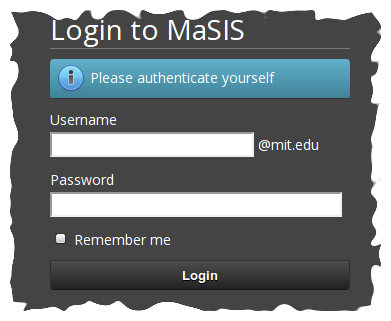
\includegraphics[width=0.6\textwidth]{screenshots/masis-login}
\caption{The login screen for MaSIS.}
\label{fig:masis-login}
\end{figure}

\index{Workspace}\marginlabel{Workspace:}
Once logged in, you will see the workspace (figure \ref{fig:masis-workspace}). This is were images are accessed, species are marked and identified, and image annotations are done. The different parts of the workspace are explained in more detail below.

\begin{figure}[hbtp]
\centering
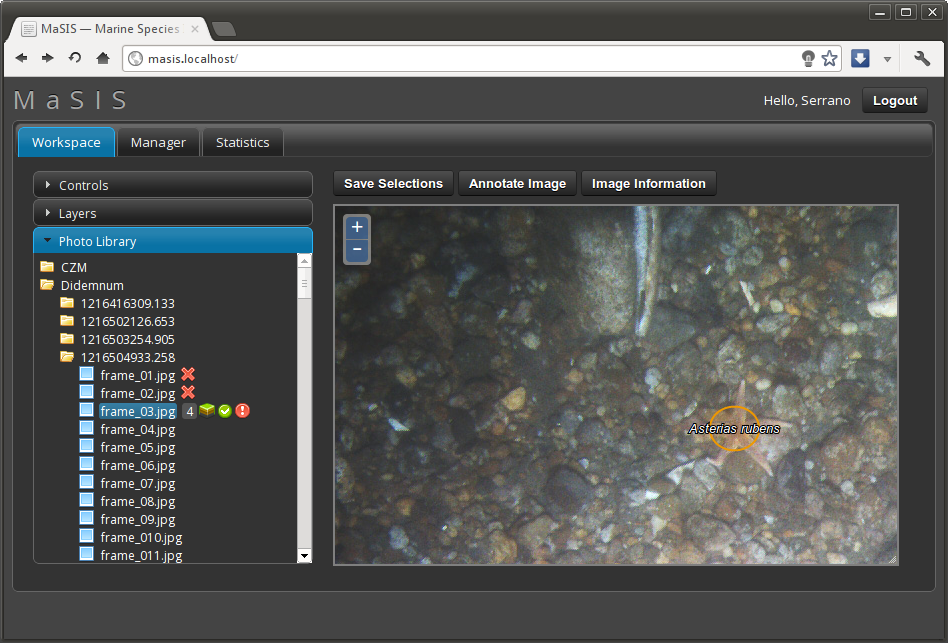
\includegraphics[width=\textwidth]{screenshots/masis-workspace}
\caption{The workspace is used to access images, mark and identify species, and annotate images.}
\label{fig:masis-workspace}
\end{figure}

\index{Photo Library}\marginlabel{Photo Library:}
In the bottom left corner of the workspace you'll find the Photo Library which displays a directory tree (figure \ref{fig:masis-photo-library}). The Photo Library is used to browse through the images that were made accessible through MaSIS. These images usually reside on the server where MaSIS is running and it does not display images from your local computer. Clicking on a directory shows the list of files for that directory. MaSIS only lists images for which meta data is set in the database. If the image has been analyzed in some ways, than this will be indicated by indicator icons on the right of the filename. Hover your mouse over an indicator icon to reveal its meaning.

\attention
The area in which the image is being loaded is by default small and you will only see a small portion of the image (the upper left portion). You can drag the gray borders or the bottom right corner of the image area to make the area larger.

\begin{figure}[hbtp]
\centering
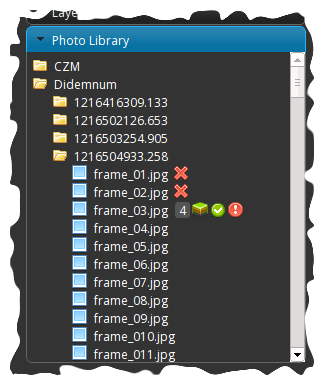
\includegraphics[width=0.5\textwidth]{screenshots/masis-photo-library}
\caption{The Photo Library is used to access and load images into the workspace.}
\label{fig:masis-photo-library}
\end{figure}

\index{Layers}\marginlabel{Layers:}
The menu on the left side of the workspace holds a Layers widget (figure \ref{fig:masis-layers}). Click on the Layers button to reveal it. Usually you'll just see two layers: the ``Base Layer'' which is the image that was loaded, and the ``Selections'' layer, which holds all the user drawn species selections. Clicking the checkbox for ``Selections'' allows you to hide and show the selections that were drawn by the user. This might be useful to have a better look at what was selected.

\begin{figure}[hbtp]
\centering
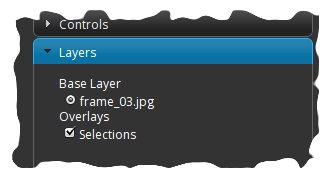
\includegraphics[width=0.5\textwidth]{screenshots/masis-layers}
\caption{The Layers widget is used to hide or show image layers.}
\label{fig:masis-layers}
\end{figure}

\index{Controls}\marginlabel{Controls:}
The menu also gives you access to the workspace controls (figure \ref{fig:masis-controls}). Controls allow you to do different things within the workspace:

\begin{figure}[hbtp]
\centering
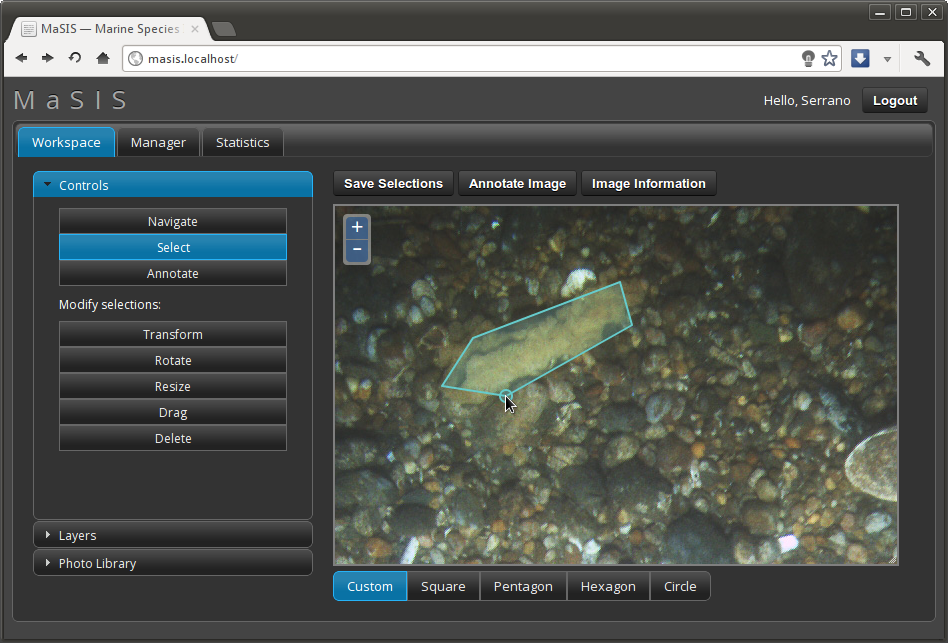
\includegraphics[width=\textwidth]{screenshots/masis-controls}
\caption{The controls are used to enable different features of the workspace.}
\label{fig:masis-controls}
\end{figure}

\begin{description}
\item[Navigate]
    The ``Navigate'' control is enabled by default when an image is loaded. It allows you to navigate the image. Simply click and hold a point within the image and drag your mouse.

\item[Select]
    The ``Select'' control allows you to mark or select organism on the image. By selecting the ``Select'' control, the select specific controls are displayed below the image (see figure \ref{fig:masis-controls}). The select control ``Custom'' is selected by default and allows you to draw custom selections (also called polygons) on the image. Alternatively, you can select ``Square'', ``Pentagon'', ``Hexagon'', and ``Circle'' which should be self-explanatory.

\item[Annotate]
    Once you have used the ``Select'' control to select organisms on the image, you can use the ``Annotate'' control to identify the organisms that you have just selected. When the ``Annotate'' control is enabled, simply click on a selection in the image to display the \nameref{Assign species dialog}. This dialog allows you to assign the selection to a species.

\item[Transform]
    The ``Transform'' control allows you to modify existing selections. Simply click on a selection to start modifying. This will display vertices on the corners of the selection. Drag the vertices to modify the selection (see figure \ref{fig:masis-modify-selection}).

\begin{figure}[hbtp]
\centering
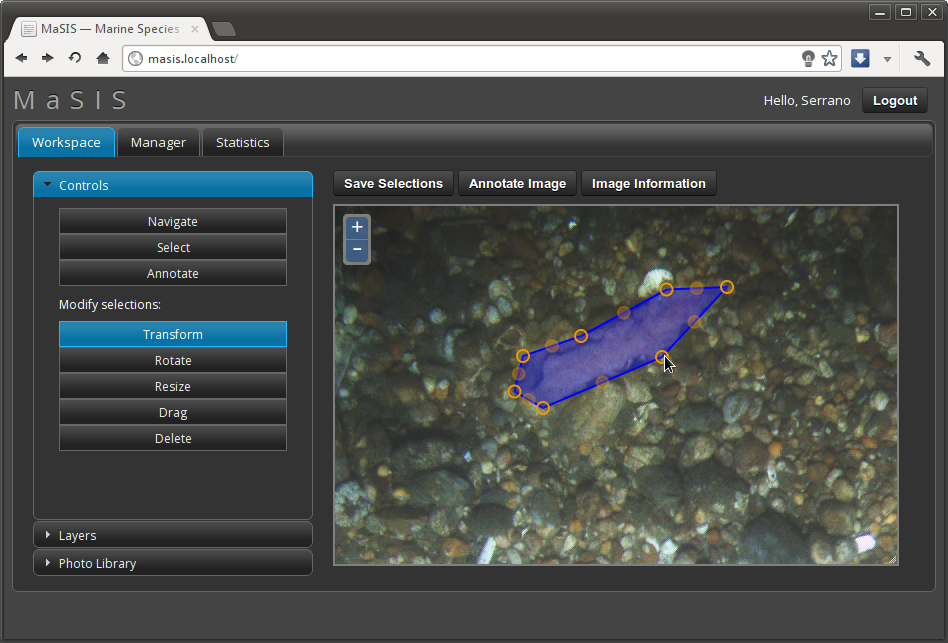
\includegraphics[width=\textwidth]{screenshots/masis-modify-selection}
\caption{Modifying a selection.}
\label{fig:masis-modify-selection}
\end{figure}

\item[Rotate]
    The ``Rotate'' control is used to rotate existing selections. Singe-click on a selection to display the rotate handler (a small circle). Then click, hold, and drag the handler to rotate.

\item[Resize]
    The ``Resize'' control is used to resize existing selections. Singe-click on a selection to display the resize handler (a small circle). Then click, hold, and drag the handler to resize.

\item[Drag]
    The ``Drag'' control is used to drag existing selections. Click, hold, and drag the selection to drag it.

\item[Delete]
    The ``Delete'' control is used to permanently delete existing selections. Click on a selection once to delete it. A confirmation dialog will be displayed to ask for a confirmation. After confirming the deletion, the selection will be immediately removed from the workspace and the database. This action is irreversible.
\end{description}

\index{Save Selections}\marginlabel{Save Selections:}
The ``Save Selections'' button above the image is used to save the selections to the database.

\attention
You will lose all your selections if you do not click this button before loading a different image, closing the web browser, or logging out. No notice is displayed when you perform an action that will result in losing your selections.

\index{Annotate Image}\marginlabel{Annotate Image:}
Clicking the ``Annotate Image'' button displays the \nameref{Annotate Image dialog}.

\index{Image Information}\marginlabel{Image Information:}
Clicking the ``Image Information'' button displays the \nameref{Image Information dialog}.

\subsubsection{Assign species dialog}
\label{Assign species dialog}

The ``Assign species'' dialog is used to assign selections to a marine species (figure \ref{fig:masis-species}). This dialog allows you to enter either the scientific name or the common name of the species. As you type the species name, the name will be matched against an online marine species database, the \href{http://www.marinespecies.org/}{World Register of Marine Species} (WoRMS). Matches are displayed in a drop-down menu and you have to select an option from the drop-down menu to assign the species. Some matches will show the label ``unaccepted'', which means that the record was marked ``unaccepted'' in the WoRMS database. Usually you should avoid assigning unaccepted species.

As matches from WoRMS are displayed, these matches are automatically saved to the local MaSIS database. You also have to option to match against species in the local database when assigning species. Matching species against the local database is much faster. Use the ``Source'' option to switch between the WoRMS database and the local database.

Once a species has been assigned, the dialog should say ``Assigned to: <species name>'' on the bottom. You can click on the species name to open the WoRMS page for that species.

To unassign a selection, search for ``Unassigned'' and click on the ``Unassigned'' option that appears.

\begin{figure}[hbtp]
\centering
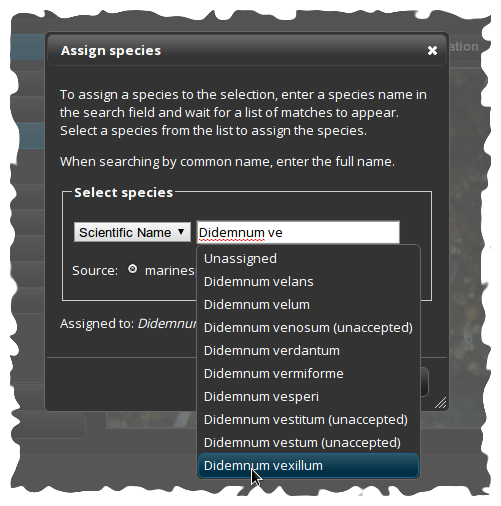
\includegraphics[width=0.6\textwidth]{screenshots/masis-species}
\caption{The Assign species dialog is used to identify marked organisms.}
\label{fig:masis-species}
\end{figure}

\subsubsection{Annotate Image dialog}
\label{Annotate Image dialog}

The Annotate Image dialog is used to annotate the image (figure \ref{fig:masis-annotate-image}). It is used to set the dominant and sub-dominant substrate types, set image tags, and set the annotation status. When the annotation status is set to ``Complete'', the species coverage data for this image is used in certain statistics (e.g. for calculating the overall species coverage).

\begin{figure}[hbtp]
\centering
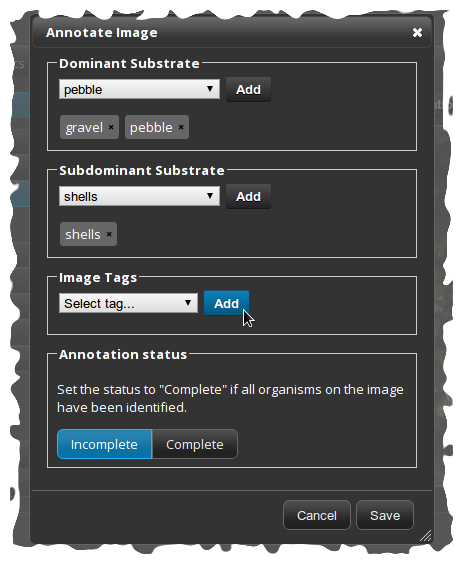
\includegraphics[width=0.6\textwidth]{screenshots/masis-annotate-image}
\caption{The Annotate Image dialog is used to annotate the substrate, set image tags, and set the annotation status.}
\label{fig:masis-annotate-image}
\end{figure}

\subsubsection{Image Information dialog}
\label{Image Information dialog}

The Image Information dialog displays the meta data for the loaded image (figure \ref{fig:masis-image-info}). Clicking the small map icon behind the location coordinates opens a new browser window with the location displayed in Google Maps.

\begin{figure}[hbtp]
\centering
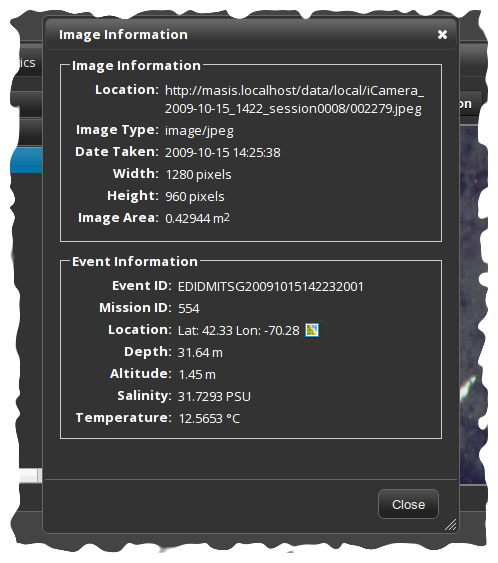
\includegraphics[width=0.6\textwidth]{screenshots/masis-image-info}
\caption{The Image Information dialog displays information for the currently loaded image.}
\label{fig:masis-image-info}
\end{figure}

\subsubsection{Manager tab}
\label{Manager tab}

The ``Manager'' tab displays tables which makes locating specific images easier (figure \ref{fig:masis-manager}).

\begin{figure}[hbtp]
\centering
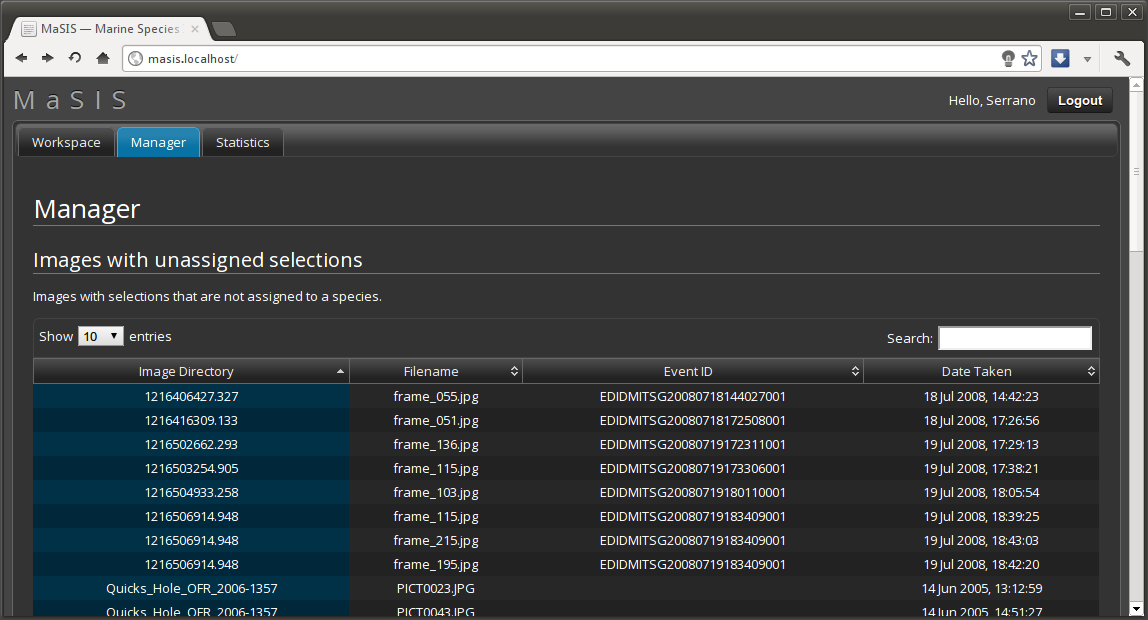
\includegraphics[width=\textwidth]{screenshots/masis-manager}
\caption{The ``Manager'' tab.}
\label{fig:masis-manager}
\end{figure}

\subsubsection{Statistics tab}
\label{Statistics tab}

The ``Statistics'' tab displays tables with general species statistics (figure \ref{fig:masis-statistics}). This page also provides a basic export feature which is used to export species percent cover data to CSV files (figure \ref{fig:masis-export}).

\begin{figure}[hbtp]
\centering
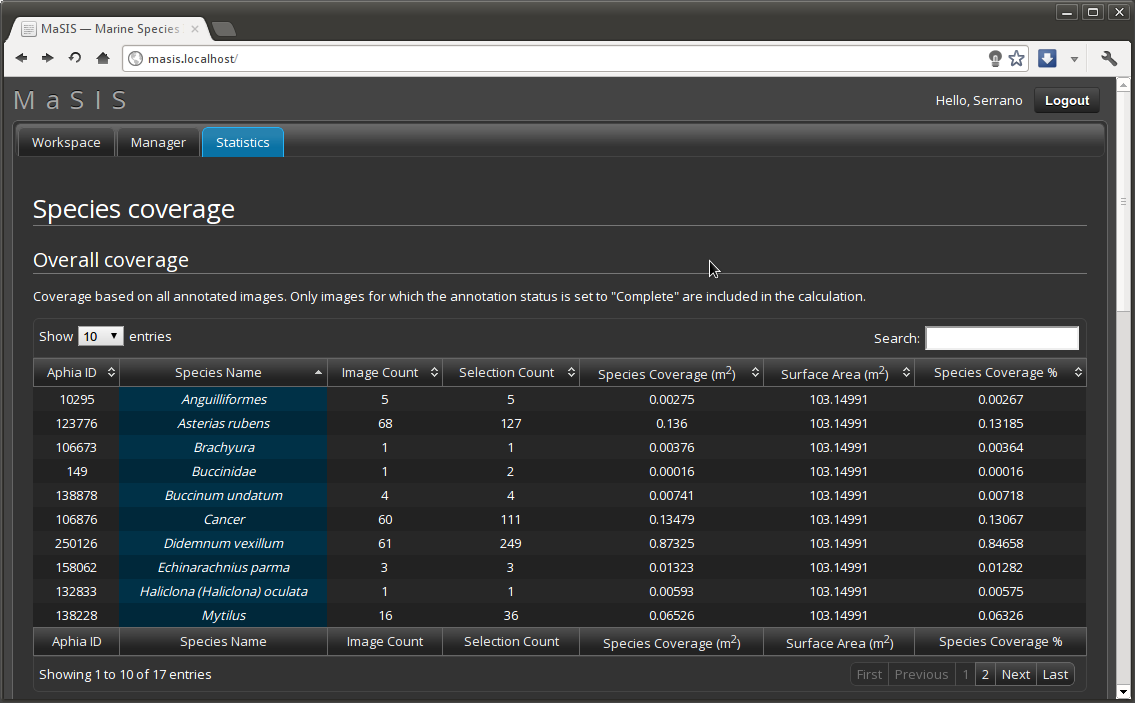
\includegraphics[width=\textwidth]{screenshots/masis-statistics}
\caption{The ``Manager'' tab.}
\label{fig:masis-statistics}
\end{figure}

\begin{figure}[hbtp]
\centering
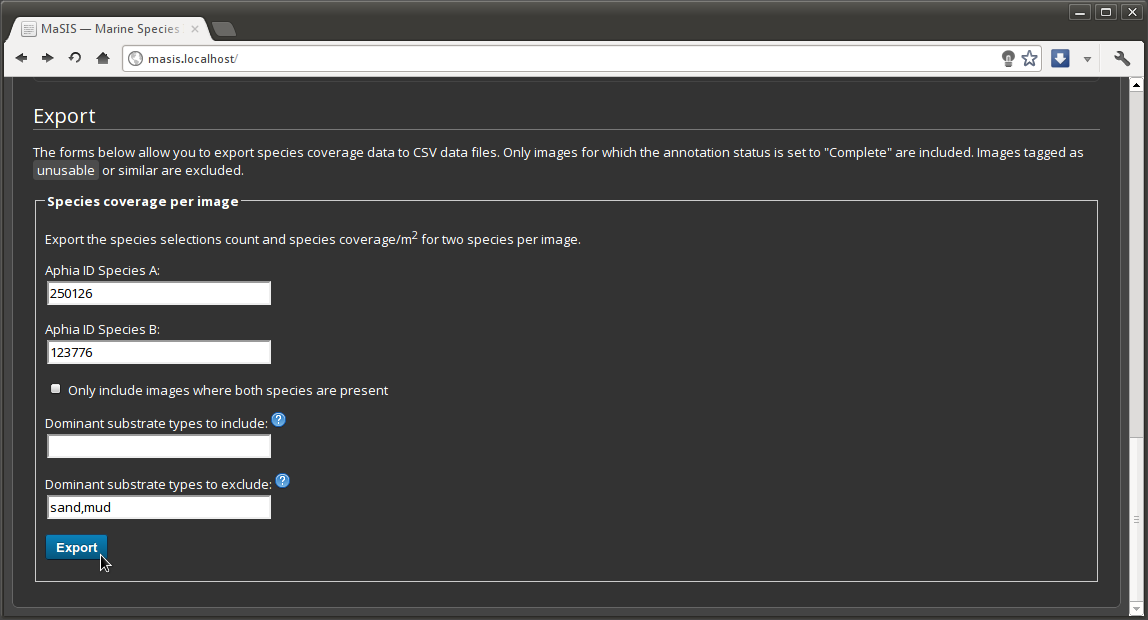
\includegraphics[width=\textwidth]{screenshots/masis-export}
\caption{The export feature.}
\label{fig:masis-export}
\end{figure}

\printindex

\end{document}
